\section{Apparato sperimentale}\label{sec:apparato-sperimentale}
\subsection{Schema del circuito}\label{subsec:schema-circuito}

GLI XOR SONO OPEN COLLECTOR => SUll'usciTA DI OGNI XOR BISOGNA AGGIUNGERE CIRCUITO DI PULLUP

%figura\begin{figure}[h]
%figura  \centering
%figura  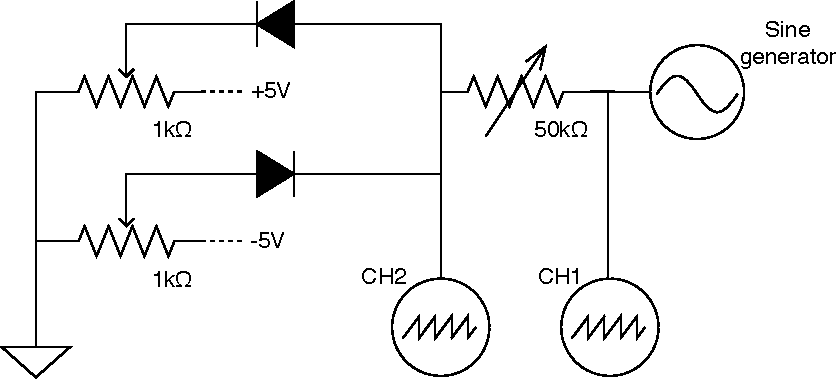
\includegraphics[width=10cm]{../assets/circuito.drawio.pdf}
%figura  \caption{
%figura    \emph{
%figura      Schema del circuito tosatore.
%figura    }
%figura  }
%figura  \label{fig:circuito}
%figura\end{figure} %todo

Il circuito che abbiamo realizzato è schematizzato in figura \ref{fig:circuito}.
È strutturato come segue:
\begin{enumerate}
  \item%
  sprema %todo
\end{enumerate}
%todo

\subsection{Materiale e strumenti usati}\label{subsec:materiali}
Segue una lista del materiale e degli strumenti usati durante la prova:
\begin{itemize}
  \item%
  Multimetro digitale, modello: \emph{ISO-TECH IDM 105}.
  \item%
  Generatore di tensione, modello: \emph{Aim-TTi EB2025T}.
  \item%
  Generatore di livelli logici, modello: \emph{Black Box}. %todo
  \item%
  Sonda per oscilloscopio.
  \item%
  Connettori vari (connettori a banana, cavi per la scheda millefori).
  \item%
  Circuiti integrati per \textsc{or}, \textsc{and}, \textsc{xor} (%todo modello).

\end{itemize}

\begin{table}[H]
  \centering
  \begin{tabular}[t]{c | c  c }
    \hline
    Grandezza & Valore & Fondoscala \\
    \hline
    d.d.p. generatore & $(5.04 \pm 0.03) \: V$ & $(20 \: V)/div$ \\
    Resistenza 1 & $(410 \pm 5) \: \Omega$ & $2 \: k\Omega$ \\
    Resistenza 2 & $(356 \pm 5) \: \Omega$ & $2 \: k\Omega$ \\
    Stato basso F.A. & $(0.12 \pm 0.01) \: V$ & $(20 \: V)/div$ \\
    Stato alto F.A. & $(4.04 \pm 0.02) \: V$ & $(20 \: V)/div$ \\
    Stato basso circ.\\ logica positiva & $(0.00 \pm 0.01) \: V$ & $(20 \: V)/div$ \\
    Stato alto circ.\\ logica positiva & $(5.04 \pm 0.03) \: V$ & $(20 \: V)/div$ \\
    \hline
  \end{tabular}
  \caption{\emph{Grandezze caratteristiche dei circuiti.}}
  \label{tab:livelli-logici}
\end{table}
